\documentclass[letterpaper,10pt]{article}
\usepackage[top=2cm, bottom=1.5cm, left=1cm, right=1cm]{geometry}
\usepackage{amsmath, amssymb, amsthm,graphicx,enumitem}
\usepackage{fancyhdr}
\pagestyle{fancy}

\lhead{\today}
\chead{MV Stats Chapter 6}
\rhead{Justin Hood}

\newcommand{\Z}{\mathbb{Z}}
\newcommand{\Q}{\mathbb{Q}}
\newcommand{\R}{\mathbb{R}}
\newcommand{\C}{\mathbb{C}}
\newtheorem{lem}{Lemma}

\begin{document}
\begin{description}
\item[6.4]\hfill \\
\begin{enumerate}[label=\alph*.]
\item We consider the analysis from example 6.1.\\
First, we take the natural log of the data in table 6.1, and perform the same analysis. First, we compute,
\[\bar{d}=\begin{bmatrix}
-0.5581951\\0.2955283
\end{bmatrix},\ S_d=\begin{bmatrix}
0.45608099 & -0.07356599\\
-0.07356599 & 0.18386750
\end{bmatrix} \]
We then consider the hypothesis test,
\begin{align*}
H_0:&\ \delta=[0,\ 0]\\
H_A:&\ \delta\neq [0,\ 0]
\end{align*}
Our $T^2$ value is then,
\[T^2=n\bar{d}'S^{-1}_d\bar{d}=10.21541\]
Next, $T^*=\frac{(n-1)p}{n-p}F_{p,n-p}(\alpha)$
\[T^*=9.458877\]
So, because $T^2>T^*$, we reject the null in favor of the alternative. So, we conclude that the difference in the two labs is not zero. We have $CI$'s,
\begin{align*}
\delta_1: &\ (-1.18444,\ 0.0680501)\\
\delta_2: &\ (-0.1020988,\ 0.6931554)
\end{align*}
\item We then construct the Bonferroni CI's as,
\begin{align*}
\delta_{b1}: &\ (-1.094488,\ -0.02190232)\\
\delta_{b2}: &\ (-0.04498455,\ 0.6360411)
\end{align*}
\item Finally, we construct the Chi-Square plot of each distance. The plot follows,
\begin{center}
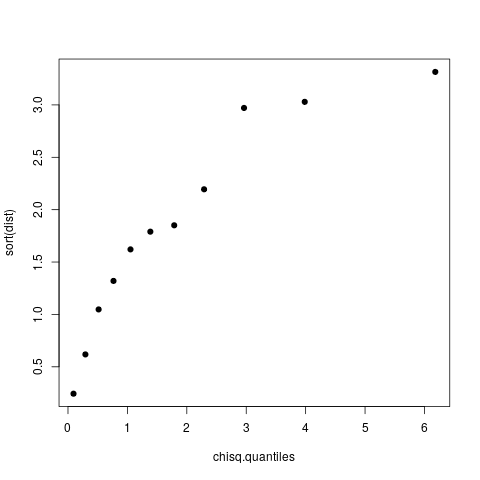
\includegraphics[scale=.75]{64chi.png}
\end{center}
From this calculation, we clearly see that the plot is not linear, and as such we have violated our normality assumptions. From the text, we note that this could be due to experimental design flaws.
\end{enumerate}
\item[6.5]\hfill \\
\begin{enumerate}[label=\alph*.]
\item We consider the data,
\[\bar{x}=\begin{bmatrix}
46.1\\57.3\\50.4
\end{bmatrix},\ S=\begin{bmatrix}
101.3 & 63.0 & 71.0\\
63.0 & 80.2 & 55.6\\
71.0 & 55.6 & 97.4
\end{bmatrix} \]
We first consider the construction of the $C$ matrix based on the equality,
\[\mu_1=\mu_2=\mu_3,\ \Rightarrow\ C=\begin{bmatrix}
1 & -1 & 0\\
0 & 1 & -1
\end{bmatrix} \]
Next, we compute,
\[T^2=n(C\bar{x})'(CSC')^{-1}(C\bar{x})=90.49458\]
and,
\[T^*=6.660417\]
Because $T^2>T^*$, we shall reject the null in facor of the alternative that the mean indices are not equal. 
\item For the construction of the simultaneous CI's, we shall append a final row onto the $C$ matrix to allow for identical computations,
\[C\to \begin{bmatrix}
1 & -1 & 0\\
0 & 1 & -1\\
-1 & 0 & 1
\end{bmatrix}\]
The intervals are then,
\begin{align*}
-14.23996 & \leq \mu_1-\mu_2 \leq -8.160045\\
3.5749 & \leq \mu_2-\mu_3 \leq 10.2251\\
1.227356 & \leq \mu_3-\mu_1 \leq 7.372644
\end{align*}
We see that none of the difference intervals contain zero, and as such we conclude that all of the means are distinct, as we expected from the test above.
\end{enumerate}
\item[6.16]\hfill \\
We consider the data from Table 4.3. We compute the $S$ matrix, and the associated $\bar{x}$ matrices,
\[\bar{x}=\begin{bmatrix}
1906.100\\1749.533\\1509.133\\1724.967
\end{bmatrix},\ S=\begin{bmatrix}
105616.30 & 94613.53 & 87289.71 & 94230.73\\
94613.53 & 101510.12 & 76137.10 & 81064.36\\
87289.71 & 76137.10 & 91917.09 & 90352.38\\
94230.73 & 81064.36 & 90352.38 & 104227.96\\
\end{bmatrix} \]
We first consider the construction of the $C$ matrix based on the equality,
\[\mu_1-\mu_2=\mu_2-\mu_3=\mu_3-\mu_4=0,\ \Rightarrow\ C=\begin{bmatrix}
1 & -1 & 0 & 0\\
0 & 1 & -1 & 0\\
0 & 0 & 1 & -1
\end{bmatrix} \]
Next, we compute,
\[T^2=n(C\bar{x})'(CSC')^{-1}(C\bar{x})=254.7212\]
and,
\[T^*=9.53891\]
Because $T^2>T^*$, we shall reject the null in favor of the alternative that the differences are nonzero. Finally, we construct the interval,
\[247.0397\leq (\mu_1+\mu_2)-(\mu_3+\mu_4)\leq 596.027\]
This interval compares the differences in both sets of means. 
\item[6.24]\hfill \\
We consider the Egyptian skull data. To begin, we partition the data into the three time periods, and obtain the following,
\begin{align*}
\bar{x}_1 &= \begin{bmatrix}
131.36667\\ 133.60000\\ 99.16667\\ 50.53333
\end{bmatrix} && S_1=\begin{bmatrix}
26.309195 & 4.1517241 & 0.4540230 & 7.2459770\\
4.151724 & 19.9724138 & -0.7931034 & 0.3931034\\
0.454023 & -0.7931034 & 34.6264368 & -1.9195402\\
7.245977 & 0.3931034 & -1.9195402 & 7.6367816
\end{bmatrix}\\
\bar{x}_2 &= \begin{bmatrix}
132.36667\\ 132.70000\\ 99.06667\\ 50.23333
\end{bmatrix}&& S_2=\begin{bmatrix}
23.136782 & 1.010345 & 4.7678161 & 1.8425287\\
1.010345 & 21.596552 & 3.3655172 & 5.6241379\\
4.767816 & 3.365517 & 18.8919540 & 0.1908046\\
1.842529 & 5.624138 & 0.1908046 & 8.7367816
\end{bmatrix}\\
\bar{x}_3 &= \begin{bmatrix}
134.46667\\ 133.80000\\ 96.03333\\ 50.56667
\end{bmatrix}&& S_2=\begin{bmatrix}
12.1195402 & 0.78620690 & -0.7747126 & 0.89885057\\
0.7862069 & 24.78620690 & 3.5931034 & -0.08965517\\
-0.7747126 & 3.59310345 & 20.7229885 & 1.67011494\\
0.8988506 & -0.08965517 & 1.6701149 & 12.59885057
\end{bmatrix}
\end{align*}
We then compute the pooled values,
\[W=\begin{bmatrix}
1785.4000 & 172.5 & 128.9667 & 289.6333\\
172.5000 & 1924.3 & 178.8000 & 171.9000\\
128.9667 & 178.8 & 2153.0000 & -1.7000\\
289.6333 & 171.9 & -1.7000 & 840.2000
\end{bmatrix},\ \bar{X}=\begin{bmatrix}
132.73333\\
133.36667\\
98.08889\\
50.44444
\end{bmatrix} \]
Next, we compute the $B$ matrix, 
\[B=\begin{bmatrix}
150.200000 & 20.300000 & -161.83333 & 5.033333\\
20.300000 & 20.600000 & -38.73333 & 6.433333\\
-161.833333 & -38.733333 & 190.28889 & -10.855556\\
5.033333 & 6.433333 & -10.85556 & 2.022222
\end{bmatrix} \]
And finally,
\[\Lambda=\frac{|W|}{|B+W|}=0.8301027\]
Noting that our critical lambda value and test statistics as,
\begin{align*}
TS &= 2.049069\\
T^* &= 1.993884
\end{align*}
Our hypotheses are,
\begin{align*}
H_0: & \tau_1=\tau_2=\tau_3=0\\
H_A: & \exists \tau_i\neq 0
\end{align*}
Because $TS>T^*$, we reject the null in favor of the alternative, that there is a diffrence between time periods.
Finally, we compute the simultaneous intervals by variable,\\\\
Max Breadth
\begin{align*}
\tau_1-\tau_2: &\ (-4.442312,\ 2.442312)\\
\tau_1-\tau_3: &\ (-6.542312,\ 0.3423115)\\
\tau_2-\tau_3: &\ (-5.542312,\ 1.342312)
\end{align*}
Bas Height
\begin{align*}
\tau_1-\tau_2: &\ (-2.673706,\ 4.473706)\\
\tau_1-\tau_3: &\ (-3.773706,\ 3.373706)\\
\tau_2-\tau_3: &\ (-4.673706,\ 2.473706)
\end{align*}
Bas Length
\begin{align*}
\tau_1-\tau_2: &\ (-3.68011,\ 3.88011)\\
\tau_1-\tau_3: &\ (-0.6467765,\ 6.913443)\\
\tau_2-\tau_3: &\ (-0.7467765,\ 6.813443)
\end{align*}
Nasal Height
\begin{align*}
\tau_1-\tau_2: &\ (-2.061423,\ 2.661423)\\
\tau_1-\tau_3: &\ (-2.394756,\ 2.328089)\\
\tau_2-\tau_3: &\ (-2.694756,\ 2.028089)
\end{align*}
We note that all of the intervals contain zero, and as such the MANOVA assumptions appear to be met. In addition, we construct our pairs plot,
\begin{center}
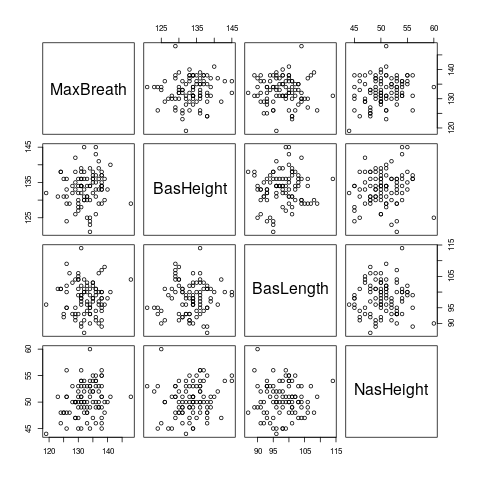
\includegraphics[scale=1]{624pair.png}
\end{center}
And note that there are no signs of correlation between the different variables.
\item[6.31]\hfill\\
We now consider the Peanut data.
\begin{enumerate}[label=\alph*.]
\item First, we perform a two factor MANOVA. Our results follow,
\begin{center}
\begin{tabular}{|r|r|r|r|r|r|}
\hline
& Df & Pillai's & F & p\\\hline
Intercept & 1 & 0.99992 & 16883.1 & $1.169e^{-8}$\\
Location & 1 & 0.89348 & 11.2 & 0.020502\\
Variety & 2 & 1.70911 & 9.8 & 0.001056\\
Location:Variety & 2 & 1.29086 & 3.0 & 0.058708\\
Residuals & 6 &&&\\\hline
\end{tabular}
\end{center}
As such, we see that based on our MANOVA in $R$, we find that both location and variety are integral to the model, but location*variety may not be.
\item Next, we analyze the QQ plots of the generated residuals as,
\begin{center}
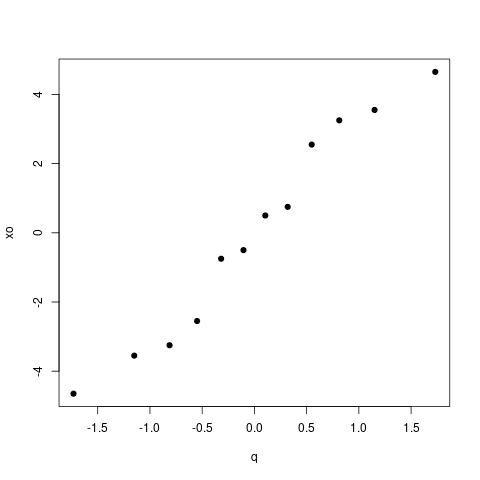
\includegraphics[scale=.5]{631r1.png}
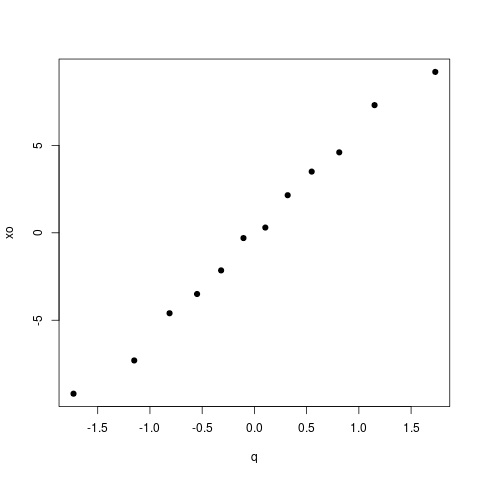
\includegraphics[scale=.5]{631r2.png}
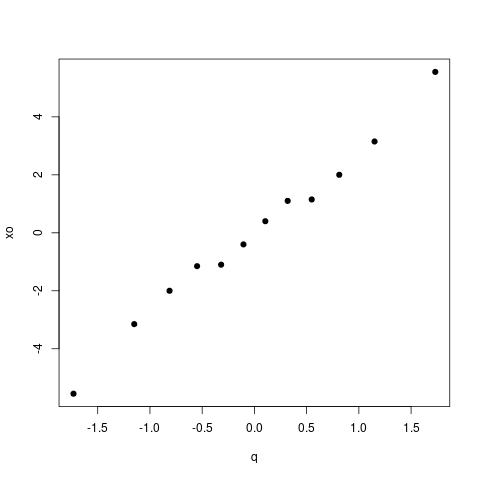
\includegraphics[scale=.5]{631r3.png}
\end{center}
We see that all of the QQ plots are linear, and as such normality cannot be rejected.
\item We see that the effects of location and variety are additive, but further information is needed regarding the interaction term. So, we perform a univariate ANOVA for each of the three response variables. For the Yield data, we get the follwing table,
\begin{center}
\begin{tabular}{|c|c|c|c|c|c|}
\hline
     &            Df & Sum Sq & Mean Sq & F value & $Pr(>F)$  \\
Location      &    1 & 0.701 &  0.701 & 0.0404 & 0.84743  \\
Variety       &    2 & 196.115 & 98.057 & 5.6460 & 0.04177 \\
Location:Variety & 2 & 205.102 & 102.551 & 5.9048 & 0.03824 \\
Residuals       &  6 & 104.205 & 17.367 &&\\\hline
\end{tabular}
\end{center}
For the SdMatKer data,
\begin{center}
\begin{tabular}{|c|c|c|c|c|c|}
\hline
       &          Df  &  Sum Sq  & Mean Sq  & F value  &  $Pr(>F)$  \\
Location      &      1   & 162.07  &  162.07  &  2.7617 &  0.14761  \\
Variety      &       2  & 1089.01 &   544.51  &  9.2786 &  0.01459 \\
Location:Variety  &  2  &  780.70  &  390.35  &  6.6517  & 0.03003 \\
Residuals    &       6  &  352.10  &   58.68  &  & \\\hline
\end{tabular}
\end{center}
For the SeedSize data,
\begin{center}
\begin{tabular}{|c|c|c|c|c|c|}
\hline
    &             Df  &  Sum Sq &  Mean Sq  & F value  &  $Pr(>F)$  \\
Location        &    1  &  72.521  &  72.521  &  4.5882 &  0.07594 \\
Variety       &      2 &  284.102 &  142.051  &  8.9872 &  0.01567\\
Location:Variety  &  2  &  85.952  &  42.976  &  2.7190 &  0.14435  \\
Residuals     &      6  &  94.835  &  15.806  &  &     \\\hline
\end{tabular}
\end{center}
From these ANOVA's we see that for the Yield and SdMatKer data the interaction term is relevant.
\item Finally, we construct the Simultaneous Bonferroni Intervals comparing the different varieties at location two as,\\
Yield,
\begin{align*}
\tau_5-\tau_6: &\ (-764.039,\ 733.839)\\
\tau_5-\tau_8: &\ (-764.639,\ 733.239)\\
\tau_6-\tau_8: &\ (-749.539,\ 748.339)
\end{align*}
SdMatKer,
\begin{align*}
\tau_5-\tau_6: &\ (-612.1639,\ 544.8639)\\
\tau_5-\tau_8: &\ (-618.5139,\ 538.5139)\\
\tau_6-\tau_8: &\ (-584.8639,\ 572.1639)
\end{align*}
SeedSize,
\begin{align*}
\tau_5-\tau_6: &\ (-540.1508,\ 525.5508)\\
\tau_5-\tau_8: &\ (-549.0008,\ 516.7008)\\
\tau_6-\tau_8: &\ (-541.7008,\ 524.0008)
\end{align*}
So, we see that zero is within each of these intervals, and there is no definite conclusion regarding variety's influence on any of the dependent variables.
\end{enumerate}
\item[6.32]\hfill \\

\end{description}
\end{document}
